\begin{frame} \frametitle{\vspace*{0.25cm} Shock-driven fluid-fluid interfaces have been studied extensively}
  {\small
    \hfill%
    \begin{figure}
      \centering
      \begin{tikzpicture}%
        \node[anchor=south west,inner sep=0] (image) at (0,0) {
          \def\svgwidth{0.6\textwidth}%
          \import{../figs/lung_figs/}{brouillette_fig3_mod_compact.pdf_tex}\hfill%
        };%
        \begin{scope}[x={(image.south east)},y={(image.north west)}]%
          \node[font=\tiny,right] at (0.15,-0.05) {\textcolor{black}{Adapted from \cite{Brouillette2002}}};%
        \end{scope}%  
      \end{tikzpicture}%
      \hfill
      \centering
      \begin{tikzpicture}%
        \node[anchor=south west,inner sep=0] (image) at (0,0) {
          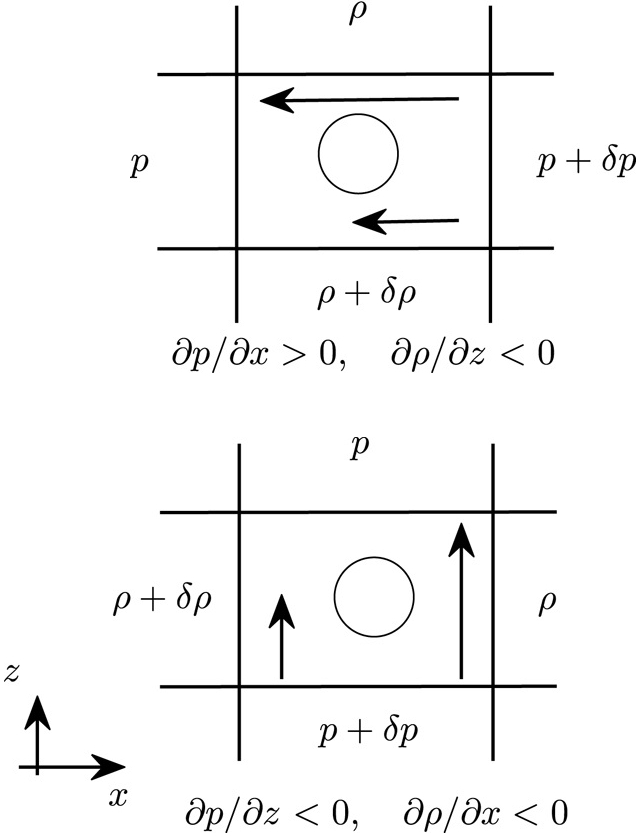
\includegraphics[height=0.5\textheight]{../figs/lung_figs/baroclinic_schematic_vertical}%
        };%
        \begin{scope}[x={(image.south east)},y={(image.north west)}]%
          \node[font=\tiny,right] at (0.05,-0.05) {\textcolor{black}{Adapted from \cite{Heifetz2015}}};%
        \end{scope}%  
      \end{tikzpicture}%
    \end{figure}
    \hfill
    \begin{itemize}
    \item Shocks deposit baroclinic vorticity at perturbed fluid-fluid interfaces \citep{Drake2006}.
    \item This vorticity drives the interface perturbation to grow.
    \item This is the Richtymyer-Meshkov ``instability''.
    \item Acoustic waves are different. They interact over a finite time-scale.
    %\item This problem is not well studied for acoustic waves.
    \end{itemize}
  }
  \note{
      {\footnotesize
      \begin{enumerate}
      \item Shock interaction with perturbed fluid-fluid interfaces has been studied.
      \item This is RM
      \item Misalignments between pressure and density gradients cause a
        local rotation in the fluid. This is called baroclinic
        vorticity.
      \item Demo with basketball: Think of this basketball as fluid
        particle, and pretend its heavier on one side than the other.
        If wind hits it, the heavier side will accelerate slower than
        the light side and the basketball will rotate.
      \item This happens at across interfaces where the density changes.
      \item This rotation in the fluid accelerates different parts of
        the perturbation in different directions, and the
        perturbation grows.
      \item Shocks take place over few molecular mfps and pass quickly.
      \item This is a mechanism that provides a way for pressure waves
        such as shocks or acoustic waves to deform a fluid-fluid
        interface.
      \item Acoustic waves are fundamentally different in that they
        their interaction with a point on the interface takes up a
        finite amount of time.
      \item And this problem isn't studies well for acoustic waves.
      \end{enumerate}
      }
    }
  \end{frame}

%%% Local Variables:
%%% mode: latex
%%% TeX-master: "../main"
%%% End:
